\section{Architecture on Google cloud} \label{sec:google}

Rubin services are built for cloud, they are scalable and use cloud deployment techniques (see \autoref{sec:deployment})

We reported on the Interim Data Facility (IDF) already at ADASS\cite{2021arXiv211115030O}, our services  have been operation on Google cloud for over three years now.
In the hybrid approach the main difference is to keep all images  and the Catalog (in Qserv) at SLAC while handling all user compute and local storage on
cloud.
In DP0.3 on IDF the Qserv instance was moved to SLAC, so we have demonstrated this also works.



\begin{figure}
\begin{centering}
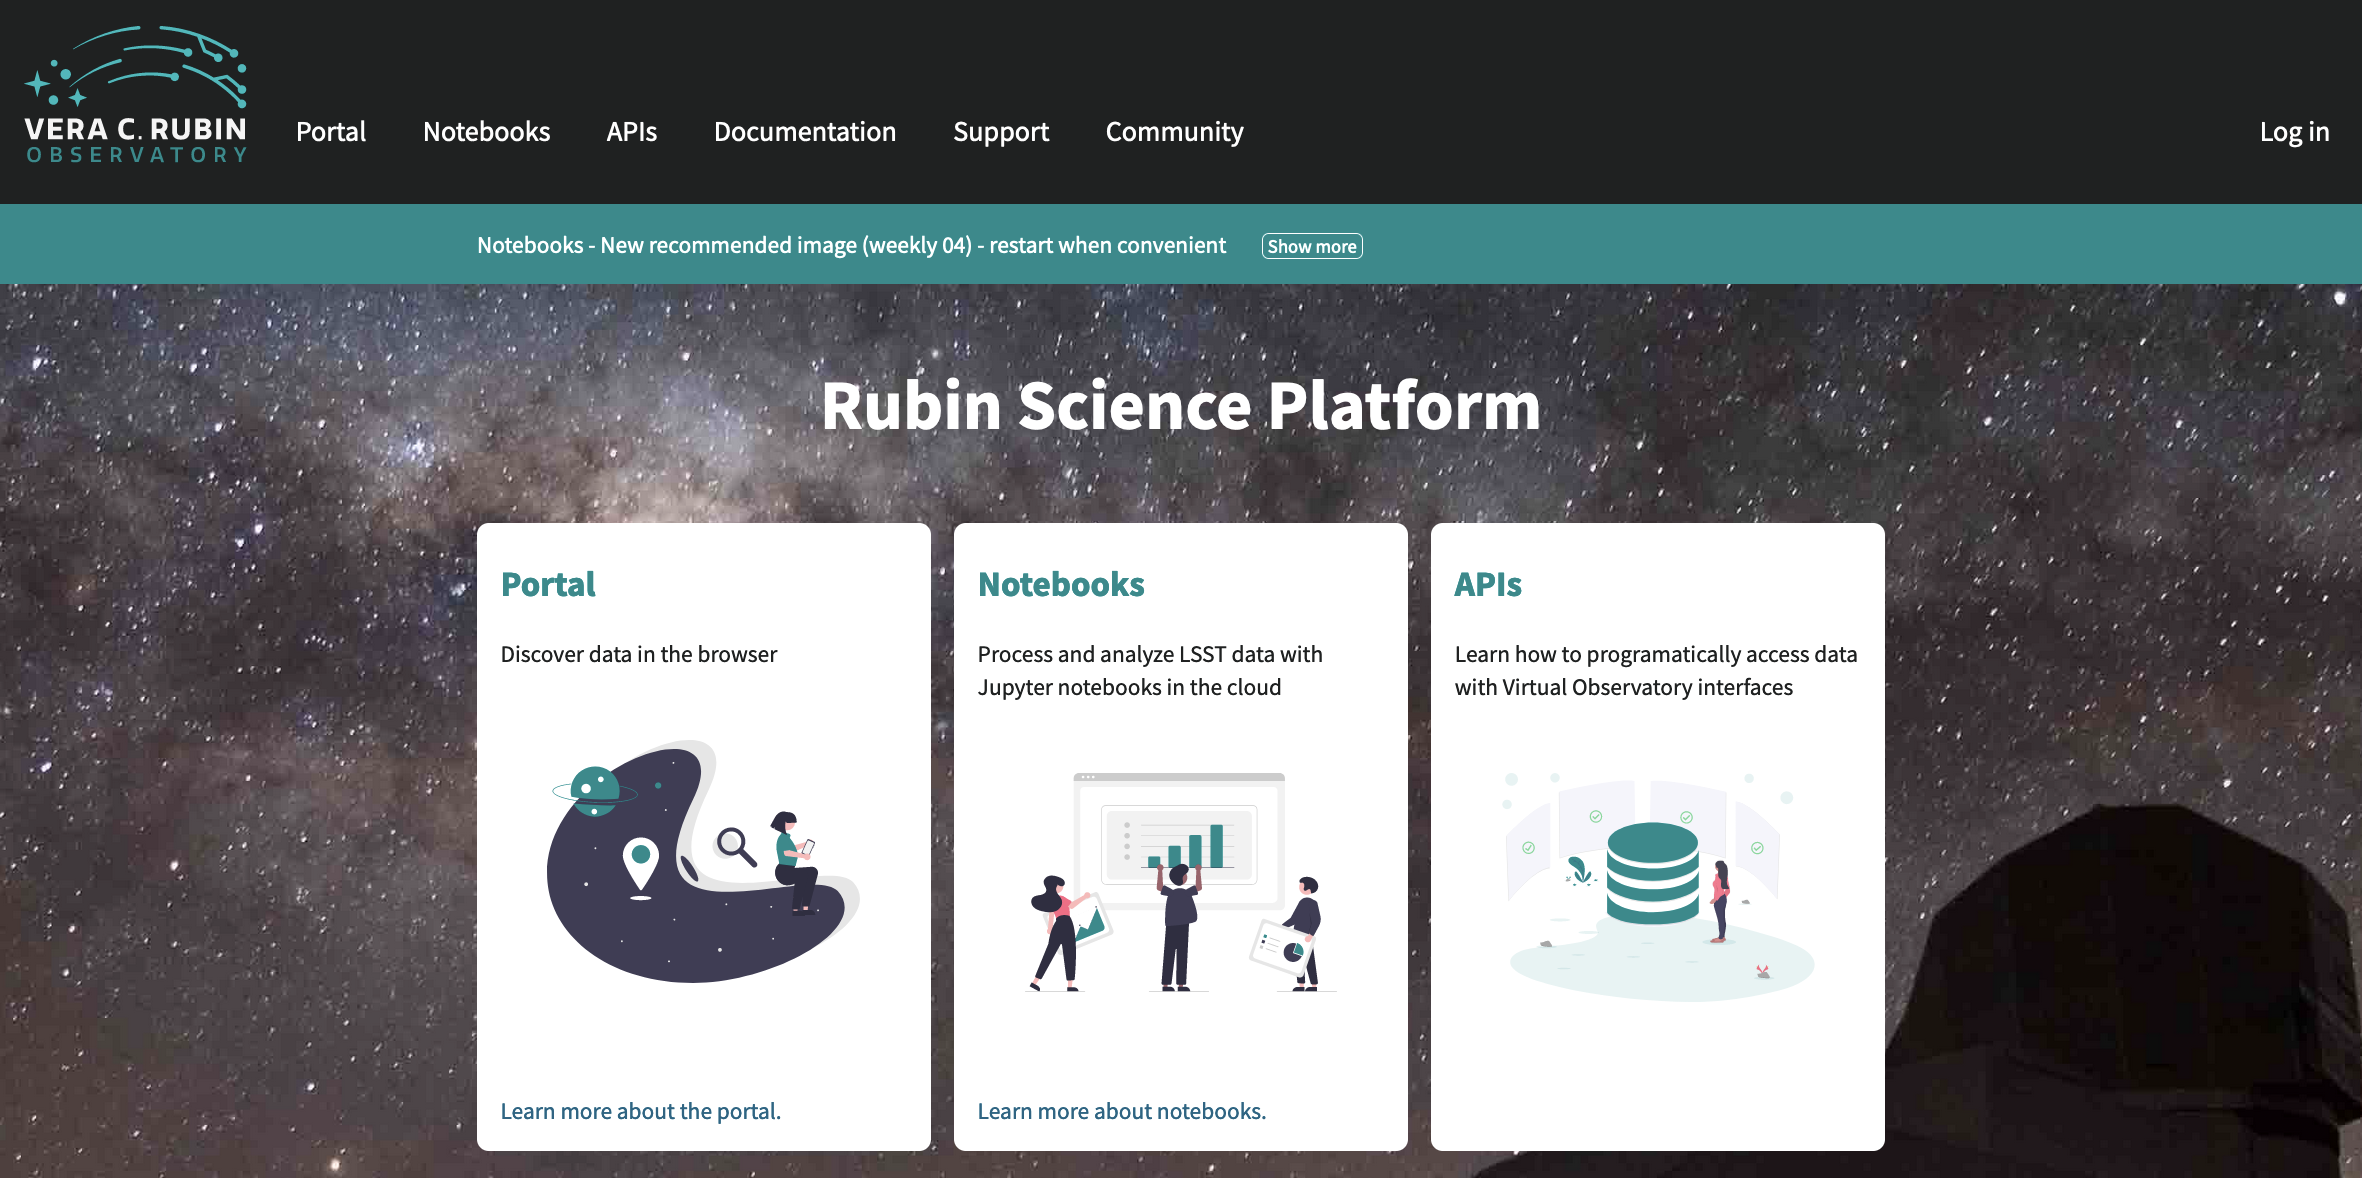
\includegraphics[width=0.9\textwidth]{RSP.png}
	\caption{ Users hosted on Google will typically use the Rubin Science Platform (RSP) depicted here.  \label{fig:goglearch}}
\end{centering}
\end{figure}


A requirement of this is the client server butler discussed  in this SPIE paper \cite{2024SPIE13101.129Jtmp}
